\documentclass[11pt]{article}

% Change "review" to "final" to generate the final (sometimes called camera-ready) version.
% Change to "preprint" to generate a non-anonymous version with page numbers.
\usepackage[preprint]{acl}

% Standard package includes
\usepackage{times}
\usepackage{latexsym}

% For proper rendering and hyphenation of words containing Latin characters (including in bib files)
\usepackage[T1]{fontenc}

% This assumes your files are encoded as UTF8
\usepackage[utf8]{inputenc}

% This is not strictly necessary, and may be commented out,
% but it will improve the layout of the manuscript,
% and will typically save some space.
\usepackage{microtype}

% This is also not strictly necessary, and may be commented out.
% However, it will improve the aesthetics of text in
% the typewriter font.
\usepackage{inconsolata}

% Additional packages
\usepackage{graphicx}
\usepackage{amsmath}
\usepackage{amssymb}
\usepackage{booktabs}
\usepackage{enumitem}
\usepackage{xcolor}
\usepackage{algorithm}
\usepackage{algpseudocode}
\usepackage{pifont}
\usepackage{multirow}
\usepackage{stfloats}

% If the title and author information does not fit in the area allocated, uncomment the following
%\setlength\titlebox{<dim>}

\author{
 \textbf{Bingxi Zhao\textsuperscript{1,2}$^*$},
 \textbf{Jiahao Zhang\textsuperscript{1}$^*$},
 \textbf{Xubin Ren\textsuperscript{1}},
 \textbf{Zirui Guo\textsuperscript{1}},
 \textbf{Chao Huang\textsuperscript{1}$^\dagger$}
\\
 \textsuperscript{1}University of Hong Kong,
 \textsuperscript{2}Beijing Jiaotong University,
\\
 \small{
   \textbf{Correspondence: \{bingxizhao39, chaohuang75\}@gmail.com} 
 }
}

\begin{document}
\title{DeepTutor: Tool-Augmented Personalized Tutoring System}
\maketitle

\begin{abstract}
\renewcommand{\thefootnote}{}%
\footnotetext{\hspace{-1.8em}$^*$Equal contribution.\newline $^\dagger$Corresponding author.}%
\renewcommand{\thefootnote}{\arabic{footnote}}%
\setcounter{footnote}{0}%
Education is one of the most promising real-world applications for Large Language Models (LLMs). However, current LLMs rely heavily on static knowledge from pre-training, and existing Retrieval-Augmented Generation (RAG) systems often prioritize retrieval precision over the adaptive, guided explanations essential for effective tutoring. 
In this paper, we present \textsc{DeepTutor}, a fully open-source agentic framework that unifies citation-grounded problem-solving with difficulty-calibrated question generation. 
These capabilities are integrated through a hybrid personalization engine that couples static knowledge grounding with a trace forest, which continuously refines evolving learner profiles to customize every interaction. 
To evaluate personalized tutoring, we construct TutorBench, featuring 100 KB-grounded customized learner profiles. 
We further conduct interactive assessments via a profile-driven student simulator, complemented by general problem-solving evaluations on authoritative benchmarks. 
Our results demonstrate that \textsc{DeepTutor} excels in personalized scenarios while maintaining robust generalized agentic abilities. 
The \textsc{DeepTutor} system and its evaluation suites are open-sourced at \url{https://github.com/HKUDS/DeepTutor}.
\end{abstract}

% ===== Sections =====
\section{Introduction}

\begin{figure}[t]
    \centering
    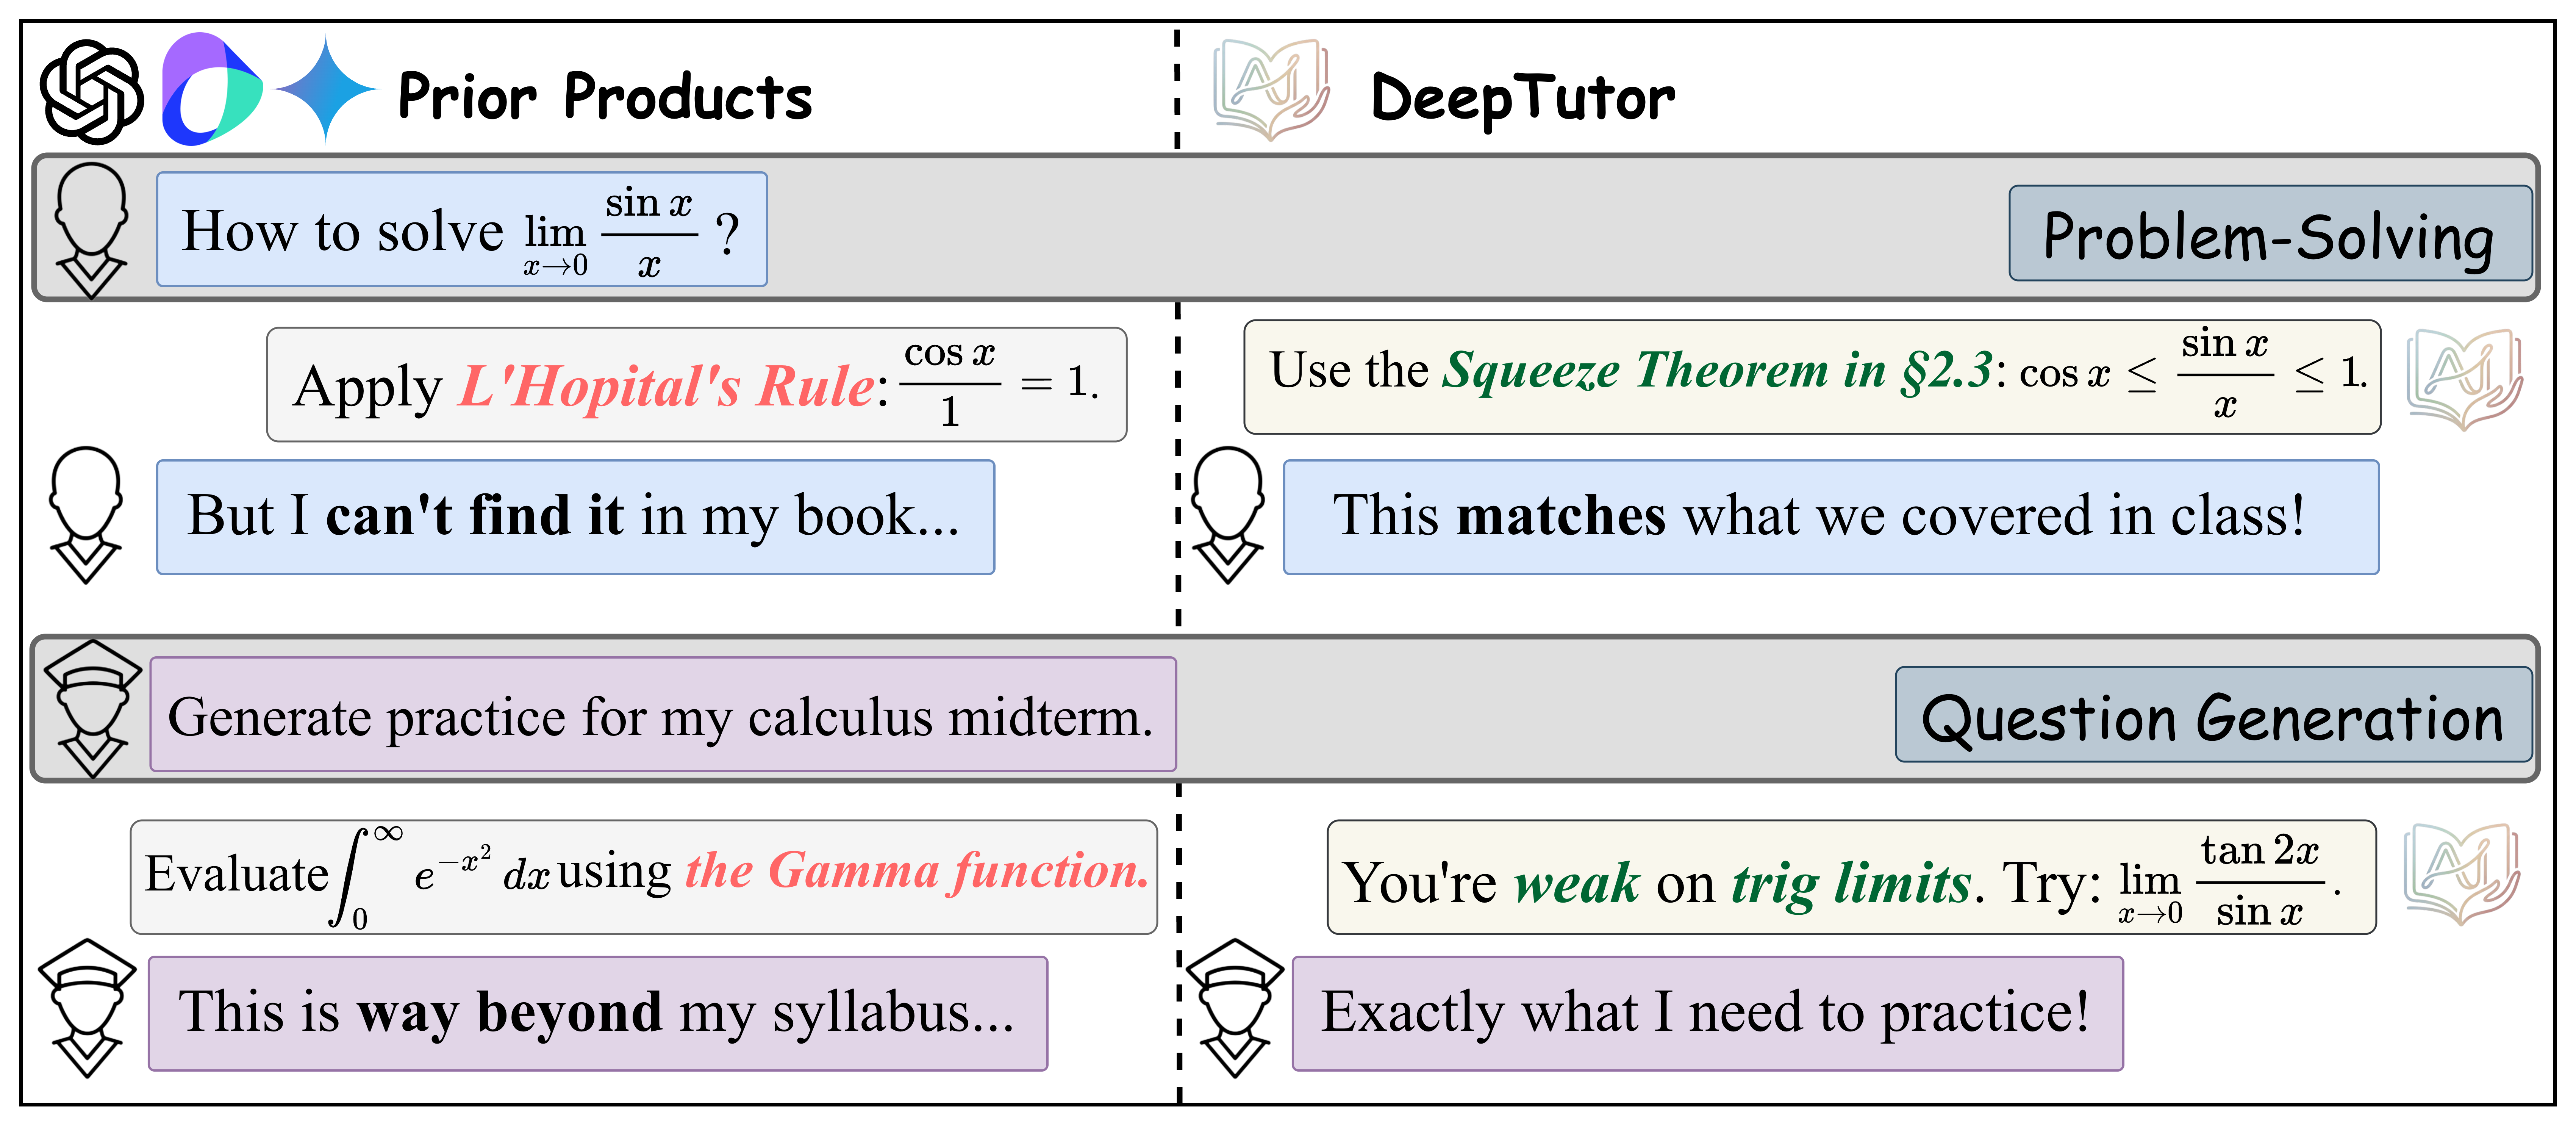
\includegraphics[width=\columnwidth]{figures/compare-ver1.png}
    \caption{Comparison of \textit{prior LLM products} and \textsc{DeepTutor}. Existing products provide generic answers regardless of the learner's background; \textsc{DeepTutor} adapts both problem-solving explanations and generated practice to match the student's syllabus, knowledge level, and specific weaknesses exposed during conversation.}
    \label{fig:compare}
\end{figure}

Education is among the most promising real-world applications of large language models (LLMs).
An effective human tutor does far more than supply correct answers--they diagnose misconceptions, scaffold explanations to the learner's level, and continuously pose targeted practice that turns weaknesses into strengths \citep{letourneau2025systematicreviewaidriven}.
While LLMs exhibit impressive fluency in educational dialogues, replicating this tightly integrated set of pedagogical skills within a unified, adaptive system remains an open challenge \citep{chu-etal-2025-llm}.

Existing approaches tackle fragments of this challenge in isolation. As illustrated in Figure~\ref{fig:compare}, the question generation of existing LLM systems rarely calibrates difficulty to the individual learner. Though SOTA LLMs demonstrate strong STEM reasoning abilities, they often tend to solve the question in a general way as they were trained. 
Question generation, on the other hand, often fails to fit the student's syllabus.
Personalized educational platforms track coarse skill inventories rather than the fine-grained reasoning traces that reveal \textit{how} a student errs.
Meanwhile, retrieval-augmented generation (RAG) often lacks consideration for the adaptive, guided explanations that effective tutoring demands.

We argue that the missing ingredient is a \textit{closed interactive loop}: weaknesses exposed during problem solving should directly shape which questions are generated next, while the learner's performance on those questions should, in turn, refine the model that informs future explanations.
This requires operationalizing personalization into measurable mechanisms, such as calibrating question difficulty based on diagnosed weaknesses and adapting explanation depth to the learner's proficiency.
Realizing such a loop requires (i)~a structured memory that captures fine-grained interaction histories rather than scalar skill scores, and (ii)~a unified tutoring system whose modules share and continuously update that memory.

To address these problems, we propose \textsc{DeepTutor} that unifies both problem solving and question generation within a hybrid personalization framework. 
For problem solving, we utilize an \textit{investigation--solving--writing} pipeline that decomposes complex queries, executes multi-step tool-augmented reasoning, and synthesizes citation-grounded explanations.
For question generation, a \textit{critic-guided generate--validate loop} iteratively proposes and verifies difficulty-calibrated practice items.
Moreover, both pipelines are unified through a hybrid personalization engine that couples static knowledge grounding with \textit{trace forest}, a dynamic structured memory that records multi-resolution interaction traces and employs specialized memory agents to continuously refine an evolving learner profile---creating the closed tutoring cycle where every interaction personalizes the next.

Our main contributions are as follows:
\begin{itemize}[nosep,leftmargin=*]
  \item We propose \textsc{DeepTutor}, an agentic tutoring framework that, to the best of our knowledge, is among the first to unify tool-augmented problem solving, critic-guided question generation, and long-term structured memory into a closed interactive loop.
  \item We introduce \textit{trace forest}, a hierarchical memory architecture in which specialized agents collaboratively maintain a fine-grained, evolving learner model from multi-resolution interaction traces.
  \item We construct \textsc{TutorBench}, a benchmark of 100 knowledge-base-grounded learner profiles paired with a student simulator for first-person interactive evaluation. Experiments on TutorBench and five standard reasoning benchmarks show that \textsc{DeepTutor} substantially outperforms various baselines, providing insights for the future shape of personalized tutoring systems.
\end{itemize}

\section{Related Work}
\label{sec:related}

\paragraph{Agentic Tool Use.}
ReAct \citep{yao2023reactsynergizingreasoningacting} introduced interleaved reasoning and action for tool-augmented LLMs, inspiring planning-and-tool workflows \citep{zhao2025llmbasedagenticreasoningframeworks,wu-etal-2025-agentic,li2025intheflowagenticoptimizationeffective}. These frameworks target short-horizon tasks without persistent learner state. DeepTutor extends tool-based agentic reasoning to stateful tutoring by coupling solving, generation, and memory.

\paragraph{Personalization and Memory.}
LLM personalization spans dialogue memory \citep{tan-etal-2025-prospect,li-etal-2025-hello,cho-etal-2022-personalized}, RAG-style adaptation \citep{li2025surveypersonalizationragagent,guo2025raganythingallinoneragframework}, and reusable workflow induction \citep{wang2024agentworkflowmemory}. Unlike traditional knowledge tracing (e.g., BKT, DKT) that maintains scalar skill scores, DeepTutor introduces Trace Forest, an event-driven structured memory that provides interpretable, multi-resolution records of learner-specific weaknesses and historical traces.

\paragraph{AI for Education.}
While classic intelligent tutoring systems (ITS) like Cognitive Tutor rely on hard-coded rules, recent LLM-based works improve personalization through conversational tutoring \citep{park2024empoweringpersonalizedlearning} and multi-agent paths \citep{wang2025llmpoweredmultiagentframeworkgoaloriented}. However, they typically rely on prompt-level adaptation without unifying solve/generate/memory loops. DeepTutor integrates tool-based reasoning, structured long-term memory, and bidirectional task coupling within a single architecture.

\section{Method}
\label{sec:method}

\begin{figure*}[t]
    \centering
    \includegraphics[width=\textwidth]{figures/full-pipe-ver7.png}
    \caption{Overview of \textsc{DeepTutor}. The system unifies two task pipelines through a Hybrid Personalization layer. \textbf{Static Knowledge Grounding} (center) constructs multi-modal knowledge graphs and vector databases from course materials, enabling mixed graph--embedding retrieval. \textbf{Dynamic Personal Memory} (bottom) maintains a trace forest accessible via a programmatic \emph{TraceToolkit}, and distills interaction histories into three evolving profile dimensions. \textbf{Personalized Problem Solving} (left) proceeds through Investigation~(\ding{172}), Step-by-step Solving~(\ding{173}), and Iterative Writing~(\ding{174}). \textbf{Personalized Question Generation} (right) proceeds via Idea Generation~(\ding{175}) and a Critic-Guided Q-A Pair Generation loop~(\ding{176}). Both pipelines record interaction traces that continuously refine the learner profile, forming a closed tutoring cycle.}
    \label{fig:overview}
\end{figure*}

DeepTutor is built around two sub-pipes with a common personalization engine, as shown in figure~\ref{fig:overview}.
The \textit{Hybrid Personalization Engine} (\S\ref{sec:personalization}) couples a static knowledge grounding---multi-modal knowledge graphs and vector databases built from course materials---with a dynamic memory that maintains an evolving learner profile.
Building upon this substrate, the \textit{problem-solving pipeline} (\S\ref{sec:solve}) produces citation-grounded explanations through three stages, while the \textit{question-generation pipeline} (\S\ref{sec:generate}) produces difficulty-calibrated practice items.
Each completed interaction feeds back into the learner profile, creating a closed tutoring cycle (\S\ref{sec:system}).

% ===========================================================================
\subsection{Preliminaries}
\label{sec:prelim}
% ===========================================================================

\paragraph{Task Formulation.}
DeepTutor addresses two complementary tutoring tasks:
(i)~\emph{problem solving}, producing a citation-grounded explanation $a$ for a learner question $q$, calibrated to the student's proficiency; and
(ii)~\emph{question generation}, producing customized practice items for a topic $\tau$ that target the learner's specific gaps.
Both tasks share the personalization substrate described below.

\paragraph{Notation.}
Course materials are indexed into a knowledge base $\mathcal{K}$ with dual representations for structured and semantic retrieval (\S\ref{sec:rag}).
The system maintains a learner profile $\mathcal{D} = (\mathcal{D}_s, \mathcal{D}_w, \mathcal{D}_r)$ capturing interaction summaries, diagnosed weaknesses, and tutor self-reflections, continuously updated by specialized memory agents (\S\ref{sec:memory}).
Before every agent step, a personalization context $\mathcal{C}_{\text{mem}}$ is assembled from $\mathcal{D}$ and the trace forest (the latter queried via a dedicated \emph{TraceToolkit}), yielding a compact, role-specific excerpt that steers the agent's behavior (\S\ref{sec:injection}).

Algorithm~\ref{alg:loop} gives a unified view of the full tutoring cycle.
Each session begins with profile injection and mixed retrieval, then branches into either problem solving (\ding{172}--\ding{174}) or question generation (\ding{175}--\ding{176}).
The resulting interaction trace is appended to the trace forest and used to update the learner profile.

\begin{algorithm}[t]
\caption{Closed-Loop Personalized Tutoring}\label{alg:loop}
\small
\begin{algorithmic}[1]
\Require learner profile $\mathcal{D}^{(0)}$;\; trace forest $\mathcal{F}^{(0)} = \emptyset$
\For{session $j = 1, 2, \ldots$}
    \State $\mathcal{C}_{\text{mem}} \gets \Call{ProfileInject}{\mathcal{D}^{(j{-}1)}, \mathcal{F}^{(j{-}1)}, \text{task}_j}$
    \State $\mathcal{C}_{\text{rag}} \gets \textsc{RagTool}(\text{task}_j)$
    \If{$\text{task}_j = (\textsc{Solve},\, q)$}
        \State $\mathcal{P}{=}\langle s_1,\dots,s_K\rangle \gets \Call{Plan}{q,\;\mathcal{C}_{\text{rag}},\;\mathcal{C}_{\text{mem}}}$ \Comment{\ding{172}}
        \For{$k = 1$ \textbf{to} $K$} \Comment{\ding{173}}
            \While{$s_k$ not resolved}
                \State $(\alpha_t,\, \mathbf{s}_t) \gets \Call{ToolAgent}{q, \mathcal{P}, \mathcal{S}, \mathcal{C}_{\text{mem}}}$
                \State $\mathcal{S} \gets \mathcal{S} \cup \{\mathbf{s}_t\}$
                \If{$\alpha_t = \textsc{Replan}$}
                    \State $\mathcal{P} \gets \Call{Revise}{\mathcal{P}, \mathcal{S}}$
                \EndIf
            \EndWhile
            \State $\mathcal{S} \gets \Call{Compress}{\mathcal{S}, k}$
        \EndFor
        \State $a \gets \Call{IterativeWrite}{\mathcal{S},\;\mathcal{C}_{\text{mem}}}$ \Comment{\ding{174}}
        \State $T_j \gets \Call{BuildTrace}{q, a}$
    \Else \Comment{$\text{task}_j = (\textsc{Generate},\, \tau)$}
        \State $\mathcal{I} \gets \Call{IdeaAgent}{\tau,\;\mathcal{C}_{\text{rag}},\;\mathcal{C}_{\text{mem}}}$ \Comment{\ding{175}}
        \State $\mathcal{T}_{1..N} \gets \Call{TopKSelect}{\mathcal{I}}$
        \For{$i = 1$ \textbf{to} $N$} \Comment{\ding{176}}
            \Repeat
                \State $(q_i, a_i) \gets \Call{Generator}{\mathcal{T}_i,\;\mathcal{C}_{\text{rag}},\;\mathcal{C}_{\text{mem}}}$
                \State $(\textit{pass}, f_i) \gets \Call{Validator}{q_i, a_i, \mathcal{T}_i}$
                \If{$\lnot\,\textit{pass}$} $\mathcal{T}_i \gets \Call{Revise}{\mathcal{T}_i, f_i}$
                \EndIf
            \Until{\textit{pass}}
        \EndFor
        \State $T_j \gets \Call{BuildTrace}{\tau, \{(q_i, a_i)\}}$
    \EndIf
    \State $\mathcal{F}^{(j)} \gets \mathcal{F}^{(j{-}1)} \cup \{T_j\}$
    \State $\mathcal{D}^{(j)} \gets \Call{MemoryUpdate}{\mathcal{D}^{(j{-}1)}, T_j}$ 
\EndFor
\end{algorithmic}
\end{algorithm}

% ===========================================================================
\subsection{Hybrid Personalization Engine}
\label{sec:personalization}
% ===========================================================================

Both the solver and the generator require two types of knowledge: \emph{domain expertise} and \emph{learner awareness}. DeepTutor provides the former through Static Knowledge Grounding and the latter through Dynamic Memory, unified by a Profile Injection mechanism that delivers tailored context to each specific stage.

\subsubsection{Static Knowledge Grounding}
\label{sec:rag}

Real-world course materials are inherently multimodal: textbooks interleave prose with figures, equations, and data tables, each encoding domain knowledge that is difficult to faithfully flatten into plain text.
To preserve this richness, we perform multimodal knowledge unification, decomposing source documents into atomic content units $\{c_j=(t_j, x_j)\}$, where $t_j\!\in\!\{\text{text}, \text{image}, \text{table}, \text{equation}\}$ denotes the modality and $x_j$ the raw payload~\cite{wang2024mineruopensourcesolutionprecise}.
Dedicated extractors handle each modality so as to retain its internal structure: figures keep their captions, equations stay anchored to surrounding definitions, and tables preserve header--cell relationships.

The resulting units are indexed through a dual-graph construction: a cross-modal KG grounds non-textual units within their contextual neighborhood via entity and relation extraction, while a text-based KG captures fine-grained semantic relationships from prose~\cite{guo2025raganythingallinoneragframework}.
The two graphs are merged through entity alignment into a unified knowledge graph $\mathcal{G}=(\mathcal{V},\mathcal{E})$ that encodes both cross-modal associations and textual semantics.
In parallel, dense encoders map all content units into modality-specific vector stores (a text VDB and a multi-modal VDB), unified into a combined embedding index $\mathcal{B}$.
Together, $\mathcal{G}$ and $\mathcal{B}$ form the complete retrieval index over the knowledge base $\mathcal{K}$.

At query time, we introduce cross-modal hybrid retrieval that operates over both indices in parallel: graph-based retrieval traverses $\mathcal{G}$ to capture explicit relationships and multi-hop reasoning paths, while embedding-based retrieval searches $\mathcal{B}$ to surface semantically relevant content beyond the graph's structural coverage.
The resulting candidate sets are merged via reciprocal rank fusion, scoring each passage $d$ as $\textstyle\sum_{r}{1}/({k+\mathrm{rank}_r(d)})$, where $k$ is a smoothing constant~\citep{cormack2009reciprocal}.
Retrieved passages are deduplicated and truncated to a context budget before injection as domain grounding $\mathcal{C}_{\text{rag}}$.

\subsubsection{Dynamic Personal Memory}
\label{sec:memory}

While the knowledge base captures \emph{what the course materials contain}, the dynamic personal memory captures \emph{how the individual learner has engaged with them}.
We further propose \textit{Trace Forest}, a structured memory $\mathcal{F} = \{T_1, T_2, \ldots\}$ in which each tree $T_j = (V_j, E_j)$ records one complete tutoring interaction as a multi-resolution, semantically searchable artifact.
Every node $v \in V_j$ is a triple $(\texttt{type}, \texttt{content}, \mathbf{e}_v)$ where \texttt{type} identifies the granularity level, \texttt{content} stores the payload, and $\mathbf{e}_v$ is a dense embedding, forming a three-level hierarchy. \textit{Level~1} captures the session-level input and a global summary; \textit{Level~2} records intermediate planning units produced by task decomposition; and \textit{Level~3} stores fine-grained execution records including tool invocations, evidence, and validation outcomes.
The concrete node types at each level are task-specific and detailed alongside the respective pipelines (\S\ref{sec:solve}, \S\ref{sec:generate}).

Rather than treating the forest as a passive data store, we expose it to all pipeline agents through a programmatic \emph{TraceToolkit} with three operations: \textsc{SearchTrace} embeds a query and retrieves the most relevant nodes across $\mathcal{F}$ via cosine similarity-based ANN search using a shared encoder; \textsc{ListTraces} enumerates traces filtered by time range, task type, or topic; and \textsc{ReadNodes} fetches the full content of specific nodes along with their ancestry path.
This interface lets each agent actively explore the learner's history with their specific demands, from coarse session summaries at Level~1 to fine-grained reasoning steps at Level~3.

\paragraph{Profile Construction.}
\label{sec:injection}
Raw traces must be interpreted into actionable tutoring signals.
We introduce three specialized memory agents to process each new trace tree $T_j$ in parallel, incrementally updating a dedicated dimension of the learner profile $\mathcal{D}$:
\begin{itemize}[nosep,leftmargin=*]
\item Session History $ \mathcal{D}_s$: distills topics covered and performance trends. This will record what has happened, providing general session memories.
\item User Weakness $\mathcal{D}_w$: compares learner responses against reference solutions, labeling each weakness as active or resolved to maintain a prioritized gap inventory, emphasizing where to focus.
\item Self-Reflection $\mathcal{D}_r$: critiques the system's own prior outputs for pedagogical alignment, producing actionable improvement notes, indicating how to improve.
\end{itemize}
Each agent receives the new trace along with its current profile dimension and produces an updated version through incremental revision. To prevent error accumulation, this process employs a \textit{confidence-gated update} mechanism, where state transitions (e.g., marking a weakness as resolved) require explicit evidence grounding, preserving long-term trends while incorporating recent signals.

Before each agent step, the system assembles a personalization context $\mathcal{C}_{\text{mem}}$ through two channels:
(i)~\emph{active trace retrieval} via the TraceToolkit, retrieving the top-$k$ most relevant nodes with $k$ allocated proportionally across levels to balance broad session context with fine-grained precedents;
(ii)~\emph{profile excerpting}, where role-specific slices of $\mathcal{D}$ are drawn based on the requesting agent's function to decouple their attention (e.g., the planner receives $\mathcal{D}_s$ and $\mathcal{D}_w$; the writer receives $\mathcal{D}_r$; generation agents receive $\mathcal{D}_w$ alongside historical question patterns). The total token budget is dynamically partitioned between $\mathcal{C}_{\text{rag}}$ and $\mathcal{C}_{\text{mem}}$ (see Appendix for a worked example).

% ===========================================================================
\subsection{Personalized Problem-Solving}
\label{sec:solve}
% ===========================================================================

Prior tool-augmented agents~\citep{yao2023reactsynergizingreasoningacting, chen2026iterresearch} pack planning, retrieval, and exposition into a full reasoning loop.
This suffices for short factoid queries but becomes a bottleneck in tutoring, where thorough investigation and personalized presentation compete for the same context budget.
DeepTutor disentangles them into three incremental stages (\ding{172}--\ding{174} in Algorithm~\ref{alg:loop}), guided by \textit{scaffolding theory} to provide step-by-step cognitive support.

\paragraph{Stage \ding{172}: Personalized Investigation.}
The planner decomposes $q$ into several meta-questions and launches a multi-source investigation: it retrieves relevant passages from $\mathcal{K}$ via the RAG tool, consults the trace forest via the trace toolkit for precedents from similar past interactions, and invokes auxiliary toolkits as needed.
Jointly conditioning on the assembled domain context $\mathcal{C}_{\text{rag}}$ and the learner context $\mathcal{C}_{\text{mem}}$, the planner produces a solving plan $\mathcal{P} = \langle s_1, \ldots, s_K \rangle$ of concrete sub-goals, each annotated with its step-level goal and a brief description.
A shared scratchpad $\mathcal{S}$ accumulates all subsequent reasoning artifacts.
Investigating before planning prevents sub-goals that are too vague or redundant with what the learner already understands (e.g., generating ``review chain rule in trigonometry'' rather than a vague ``review calculus'').

\paragraph{Stage \ding{173}: Step-by-step Problem Solving.}
Each sub-goal $s_k$ is executed through a ReAct-style loop, ~\citep{yao2023reactsynergizingreasoningacting}, conditioned on both the domain grounding $\mathcal{C}_{\text{rag}}$ and the learner context $\mathcal{C}_{\text{mem}}$.
At every iteration the tool agent produces a reasoning trace $r_t$, selects an action $\alpha_t$ from a shared tool suite $\mathcal{A}$ (encompassing knowledge-base retrieval, trace-forest lookup, sandboxed code execution, web search, and deep reasoning), observes the output $o_t$, and records a \emph{self-note} $n_t$.
Unlike the reasoning trace, which captures the full deliberation process, the self-note distills the step's outcome into a concise takeaway (e.g., ``retrieved formula confirmed'') that subsequent steps can reference without re-reading verbose intermediates.
When the current plan proves inadequate, the agent triggers \emph{adaptive replanning}, revising remaining sub-goals while preserving completed work.

Hierarchical compression (line 14 in Algorithm~\ref{alg:loop}) prevents the scratchpad from exceeding the model's context window.
Once sub-goal $s_k$ is resolved, an LLM-based summarizer distills its full trace into a compact digest that retains key conclusions and evidence pointers while discarding verbose intermediate steps.
As the plan advances, earlier sub-goals are represented by increasingly concise digests, freeing context capacity for deeper reasoning on later sub-goals.

\paragraph{Stage \ding{174}: Evidence-based Iterative Writing.}
Rather than concatenating raw tool outputs, the writing stage extracts structured evidence bundles from the scratchpad and constructs the answer through successive draft-refine iterations, reconciling potentially conflicting findings.
The learner context $\mathcal{C}_{\text{mem}}$
% ---including diagnosed weaknesses from $\mathcal{D}_w$ and the system's pedagogical self-reflections from $\mathcal{D}_r$---
steers both the depth and the tone of the explanation within the learner's \textit{Zone of Proximal Development}: \textit{beginners} receive step-by-step derivations with scaffolding, while \textit{proficient learners} receive focused summaries that foreground key insights.
Every claim is grounded with traceable citations back to $\mathcal{K}$.

% ===========================================================================
\subsection{Personalized Question Generation}
\label{sec:generate}
% ===========================================================================

A tutor must also pose the right questions: ones that are meaningful, factually grounded, and calibrated to the individual learner.
We propose a two-stage architecture (\ding{175}--\ding{176} in Algorithm~\ref{alg:loop}) that separates \emph{what to ask} from \emph{how to ask and verify}.

\paragraph{Stage \ding{175}: Personalized Idea Generation.}
Rather than generating questions directly from a bare topic, DeepTutor first maps the conceptual landscape around $\tau$ through the lens of the individual learner.
The idea agent jointly conditions on domain knowledge $\mathcal{C}_{\text{rag}}$ and learner context $\mathcal{C}_{\text{mem}}$---including past mistakes, difficulty trends, and related problems surfaced via the TraceToolkit---to synthesize a diverse pool of candidate ideas, each characterized by a target concept, a question format (MCQ, written-response, or coding), and a personalized rationale grounded in the learner's diagnosed gaps.
A two-stage selection then filters ill-formed or redundant candidates and ranks survivors along quality dimensions such as clarity, relevance, and diversity, yielding structured question templates $\{\mathcal{T}_i\}$ that serve as blueprints for the subsequent generation stage.

\paragraph{Stage \ding{176}: Critic-Guided Q-A Pair Generation.}
For each template $\mathcal{T}_i$, a \textbf{generator} produces a complete question--answer--explanation triple $(q_i, a_i, e_i)$, drawing on $\mathcal{C}_{\text{rag}}$ for factual grounding and $\mathcal{C}_{\text{mem}}$ to calibrate difficulty and phrasing to the learner's level.
A structurally separated \textbf{validator} then challenges the output through two-level quality assurance: an LLM-based reasoning check evaluates template alignment, factual correctness, and pedagogical soundness, while computational questions undergo additional verification via sandboxed code execution.
This dual-agent separation is critical: because the validator shares no reasoning chain with the generator, it must independently verify correctness, catching errors that self-evaluation would miss.
Failed pairs receive structured diagnostic feedback $f_i$; the template is revised and the pair regenerated until both pedagogical and factual constraints are satisfied.

% ===========================================================================
\subsection{Closed-Loop Tutoring Cycle}
\label{sec:system}
% ===========================================================================

As shown in Algorithm~\ref{alg:loop}, the components above form a self-reinforcing cycle.
After each task, whether a problem-solving session or a question-generation episode, the pipeline records a new trace tree $T_j$ into the trace forest $\mathcal{F}$, and the three memory agents update the learner profile in parallel, producing $\mathcal{D}^{(j)}$ that immediately informs subsequent interactions.
The key property is \textbf{bidirectional task coupling}, which operationalizes \textit{formative assessment}: weaknesses diagnosed during problem solving propagate to $\mathcal{D}_w$ and directly shape which questions are generated next; conversely, the learner's performance on generated questions refines $\mathcal{D}_s$ and $\mathcal{D}_r$, improving future explanations.
Because every agent can actively query the trace forest through the TraceToolkit, this feedback is not limited to profile-level summaries: agents can retrieve fine-grained precedents from any prior interaction, enabling increasingly nuanced personalization as the interaction history grows.

    % ===========================================================================
    % Section 4: Experiments
    % ===========================================================================
    
    \begin{figure*}[htbp!]
      \centering
      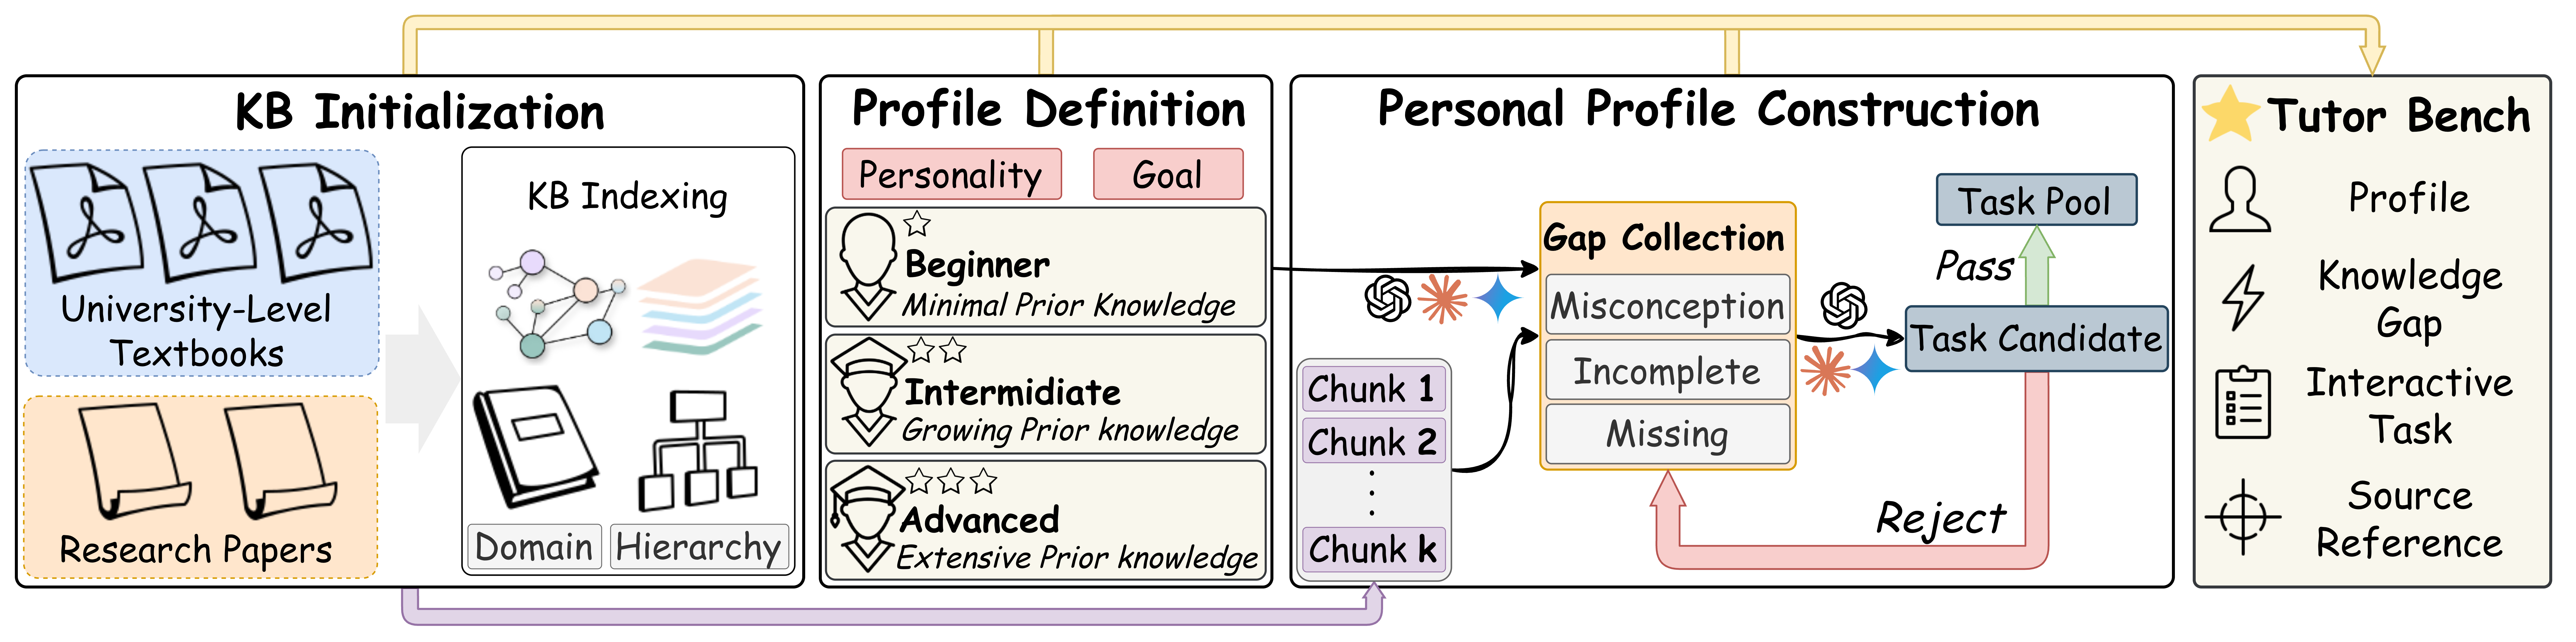
\includegraphics[width=\textwidth]{figures/data-gen-ver2.png}
      \caption{Construction pipeline of \textbf{TutorBench}. Four stages---KB Initialization, Profile Definition, Personal Profile Construction (with grounded knowledge gaps and rejection sampling), and final assembly---produce entries each containing a learner profile, knowledge gaps, an interactive task, and source references.}
      \label{fig:datagen}
  \end{figure*}
  
  
  \section{Experiments}
  \label{sec:experiments}
  
Conventional QA-style benchmarks mostly measure final correctness, but personalized tutoring requires process-level evaluation: whether the system diagnoses learner-specific gaps, corrects them through interaction, and then generates targeted follow-up practice.
Accordingly, we evaluate \textsc{DeepTutor} along three axes:
\textbf{TutorBench} construction quality (\S\ref{sec:tutorbench}),
\textbf{first-person interactive tutoring quality} (\S\ref{sec:interactive_eval}),
and \textbf{general problem-solving transfer} (\S\ref{sec:generalization}).
  
  
  % ===========================================================================
  \subsection{TutorBench: A Personalized Tutoring Benchmark}
  \label{sec:tutorbench}
  % ===========================================================================
  
Existing educational benchmarks rarely model who the student is and what they specifically misunderstand.
We construct \textbf{TutorBench}, where each entry explicitly couples a learner persona, grounded knowledge gaps, and an interactive tutoring task.
The construction pipeline is shown in Figure~\ref{fig:datagen}.
  
  \paragraph{KB Initialization.}
  University-level textbooks and research papers are indexed into the dual-representation knowledge base described in \S\ref{sec:rag}.
  A \textit{domain hierarchy} is simultaneously derived from the document structure, providing topical scaffolding for subsequent profile generation.
  
\paragraph{Profile Definition.}
Each KB instantiates three learner profiles---\textit{beginner}, \textit{intermediate}, and \textit{advanced}---with distinct educational background, learning purpose, and per-topic mastery states (\textit{known well}/\textit{partially known}/\textit{unknown}).
This mirrors the benchmark generator configuration used in the codebase.
  
\paragraph{Personal Profile Construction.}
For each profile, we sample source pages from the KB and generate three types of \emph{grounded knowledge gaps}:
  \textbf{misconceptions} (incorrect beliefs),
  \textbf{incomplete understanding} (partial grasp with missed edge cases), and
  \textbf{missing knowledge} (never-encountered concepts).
  Each gap is anchored to specific source pages and includes both a \textit{manifestation} (how the student would exhibit the gap) and the \textit{correct understanding} for evaluation reference.
  
Gaps are assembled into \textbf{interactive tasks} via rejection sampling that verifies task--gap consistency, source grounding, and conversational naturalness.
  
\paragraph{Statistics.}
TutorBench is generated with a fixed, configuration-driven recipe.
For each KB, we instantiate three learner profiles (\textit{beginner},
\textit{intermediate}, \textit{advanced}), yielding $3 \times N_{\text{KB}}$
profiles in total. We sample source pages to generate at least 3 knowledge gaps for each interactive task and construct 3
interactive tasks per profile via rejection sampling. In our current release, this produces 90 KB-grounded learner
profiles overall, which is 270 interactive tasks.
  
  
  % ===========================================================================
  \subsection{First-Person Interactive Evaluation}
  \label{sec:interactive_eval}
  % ===========================================================================
  
Static evaluation cannot capture whether a tutor adaptively resolves misconceptions over turns.
We therefore use a \textbf{first-person interactive protocol}: an LLM student simulator (initialized from TutorBench entries) interacts with each evaluated system, and we score both dialogue behavior and generated practice questions (Figure~\ref{fig:evaluation}).
  
  \begin{figure}[t]
      \centering
      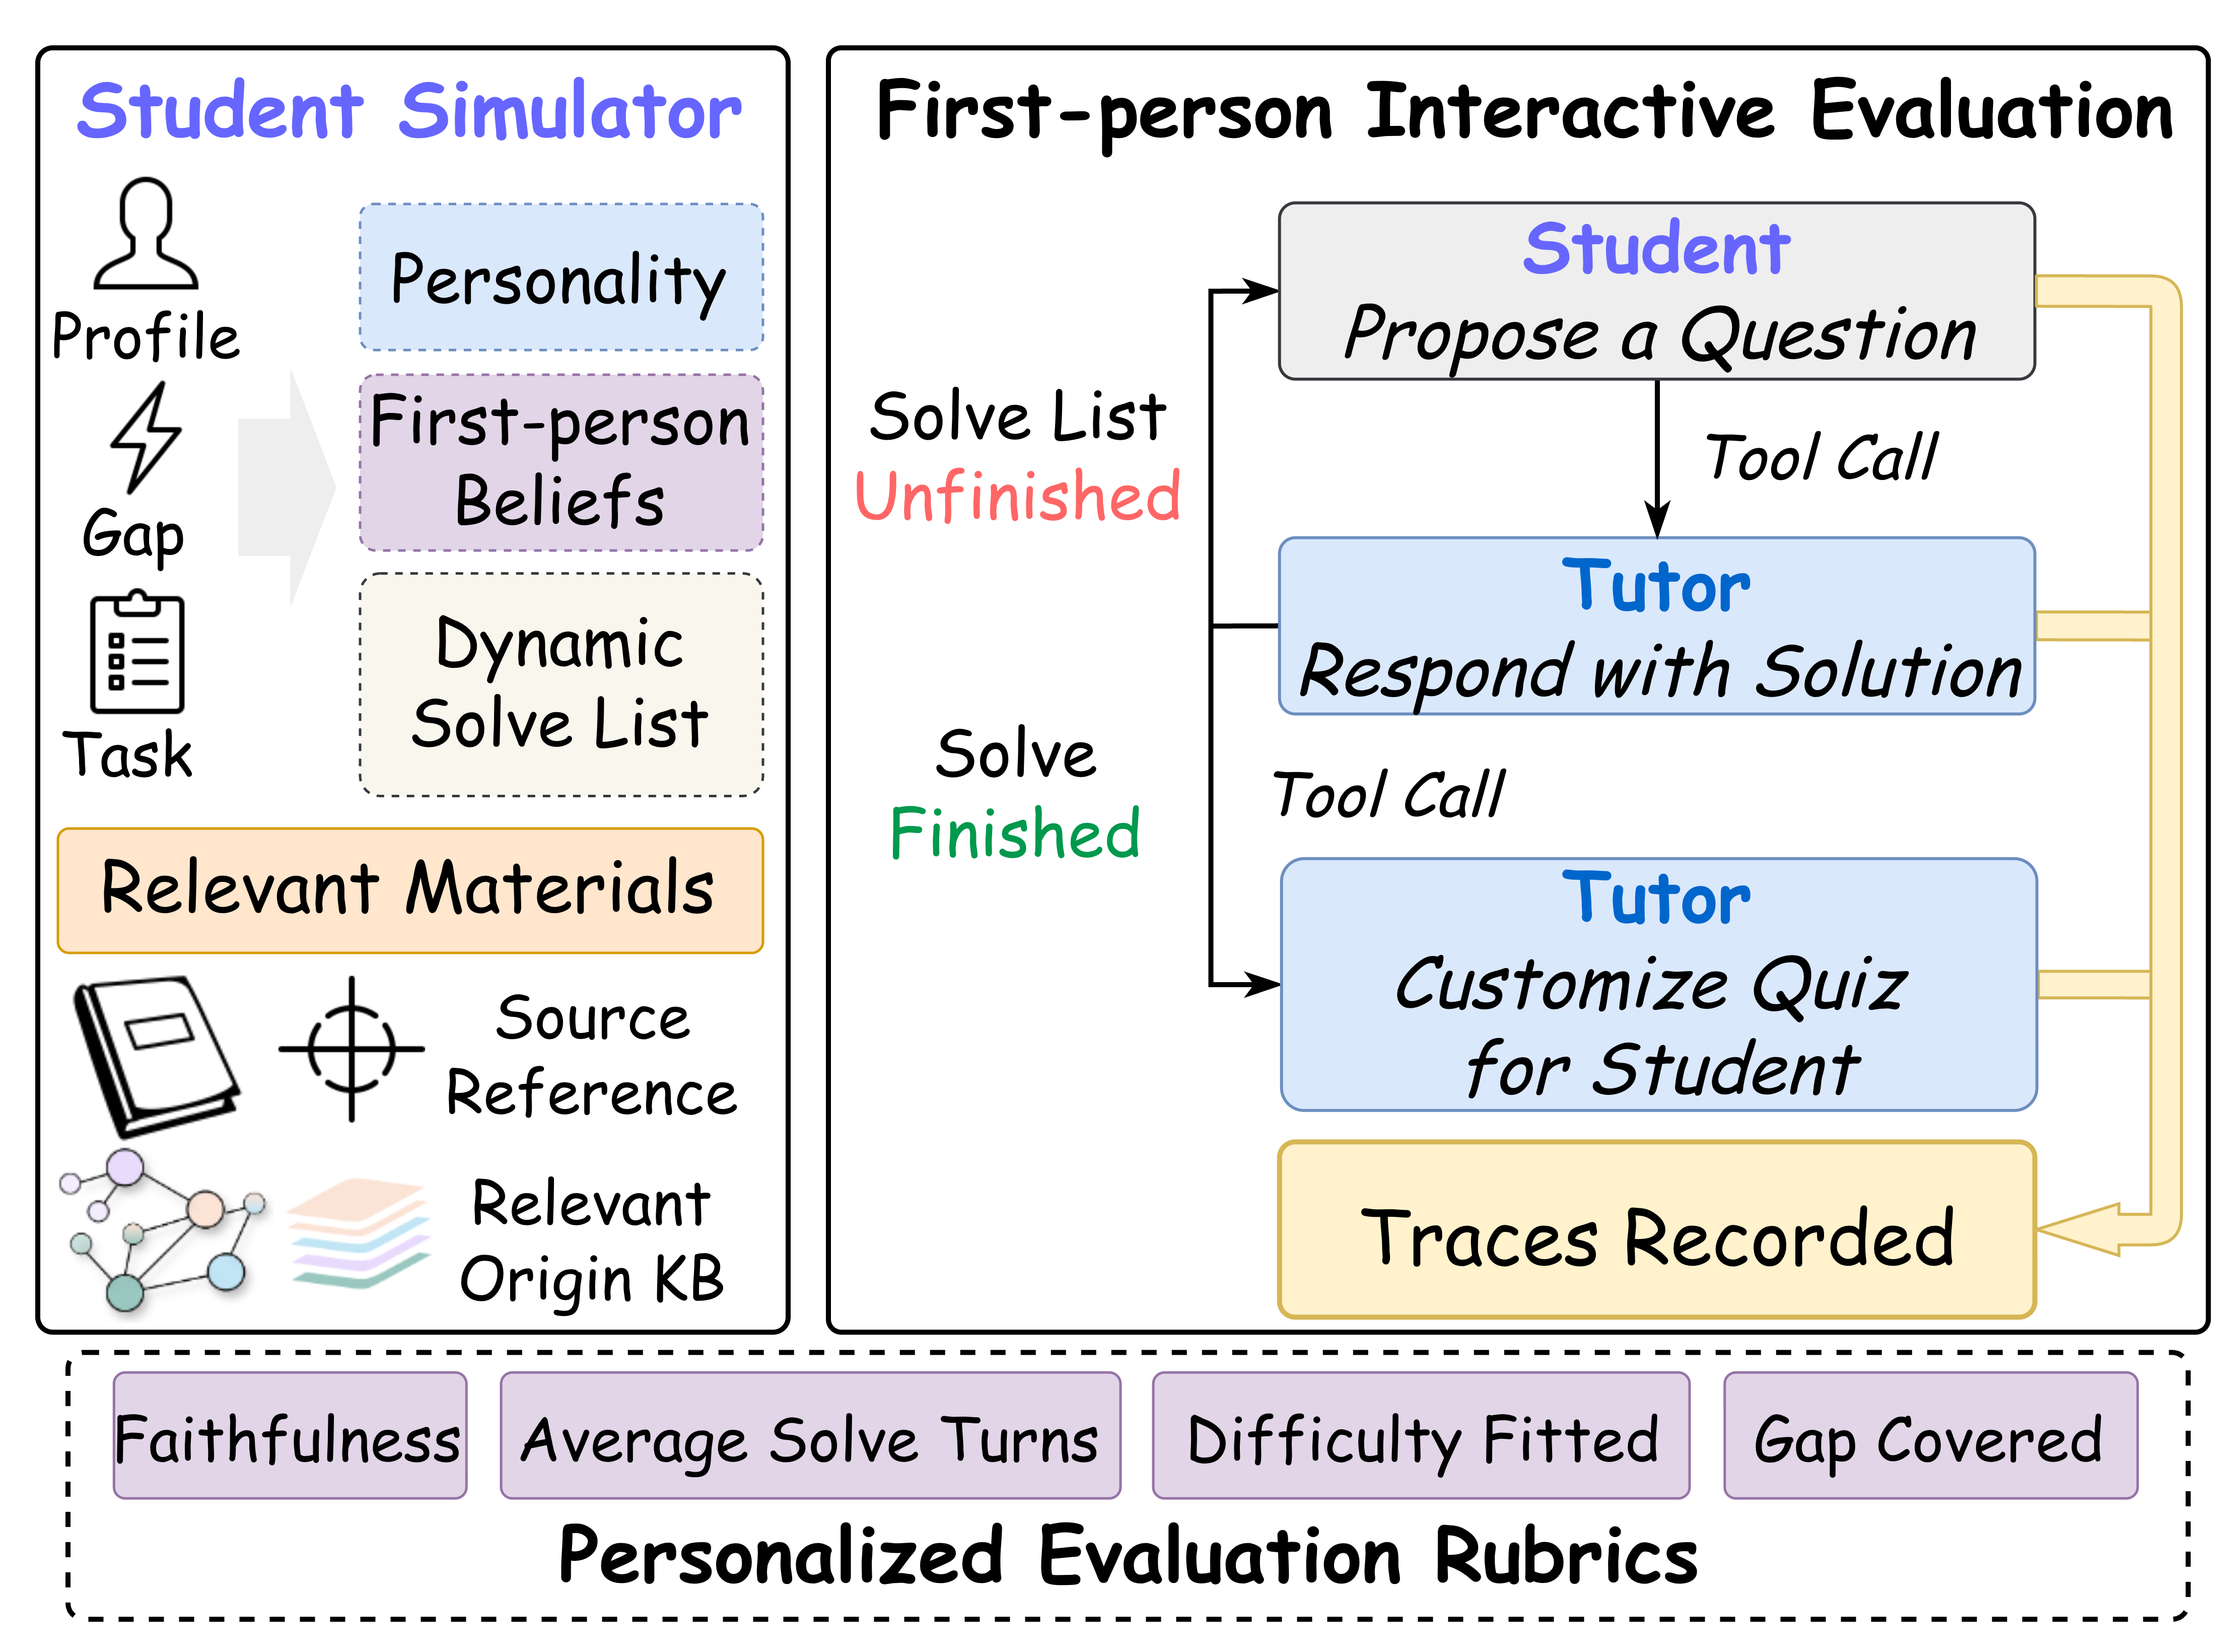
\includegraphics[width=\columnwidth]{figures/evaluation-ver1.png}
    \caption{First-person interactive evaluation protocol. A \textbf{Student Simulator} initialized from TutorBench (persona + first-person gap beliefs + dynamic gap pacing) interacts with the tutor. After session completion, the tutor generates five practice questions. Evaluation is split into \textbf{turn-level tutoring metrics} and \textbf{practice-question metrics}, then aggregated in a fixed-judge Step-3 pipeline.}
      \label{fig:evaluation}
  \end{figure}
  
\paragraph{Student Simulator.}
Each gap is transformed into a first-person belief so the simulator \emph{acts as the student} rather than describing errors from an outside view.
Combined with dynamic gap pacing, this yields realistic resistance patterns: the student may defend misconceptions, partially accept corrections, and only mark completion after sufficient explanation.
  
\paragraph{Evaluation Rubrics.}
Following the latest evaluation pipeline, metrics are explicitly split into
\textbf{turn-level tutoring metrics} and \textbf{practice-question metrics}.
Importantly, the final practice-question turn is \emph{excluded} from turn-level scoring and evaluated independently.
  
  \begin{itemize}[nosep,leftmargin=*]
\item \textbf{Iter}: raw turn count from interactive sessions (lower is better). This is the only non-1--5 metric.
  
\item \textbf{Solve-side Quality}: per-turn 1--5 scores for \textit{personalization}, \textit{applicability}, \textit{source faithfulness}, \textit{vividness} (modality diversity of expression, e.g., structured tables when useful), and \textit{logical depth}.
  
\item \textbf{Practice Metrics}: after dialogue ends, five generated \textbf{MCQ} questions are evaluated separately:
\textit{fitness}, \textit{groundedness}, \textit{diversity}, \textit{answer quality}, and \textit{cross concept} (all per-question, all 1--5).
  \end{itemize}
  
  \paragraph{Protocol.}
We run a three-stage pipeline:
\textbf{Step 1} generates benchmark entries,
\textbf{Step 2} runs interactive simulation and logs transcripts,
\textbf{Step 3} scores transcripts with LLM-as-judge prompts.
To ensure comparability in model studies, we support multi-model Step-2 generation while fixing a single judge model in Step-3.
We compare \textbf{\textsc{DeepTutor}} against one baseline:
\textbf{Naive Tutor} (the project mock tutor: base LLM + simple RAG, without structured planning/memory loop).
  
  \paragraph{Results.}
Table~\ref{tab:interactive_results_main} reports the main interactive metrics used in the paper body.
Table~\ref{tab:interactive_results_full} provides the extended metric breakdown (turn-level teaching quality and additional practice-quality dimensions).
Across our internal runs, \textsc{DeepTutor} consistently improves both tutoring and practice metrics over \textit{Naive Tutor}. For all 1--5 metrics, we report averages with four decimal places.
  
  \begin{table}[t]
  \centering
  \small
  \begin{tabular}{lcccc}
  \toprule
  \textbf{System} & \textbf{SQ}$\uparrow$ & \textbf{PQ}$\uparrow$ & \textbf{OQ}$\uparrow$ & \textbf{Iter}$\downarrow$ \\
  \midrule
  Naive Tutor          & --  & --  & --  & -- \\
  \textsc{DeepTutor}   & --  & --  & --  & -- \\
  \bottomrule
  \end{tabular}
\caption{Main first-person interactive results. SQ: solve-quality composite over \{SF, personalization, applicability, vividness, logical depth\}. PQ: practice-quality composite over \{fitness, groundedness, diversity, answer quality, cross concept\}. OQ: average of SQ and PQ. Iter: raw turn count (lower is better).
  }
  \label{tab:interactive_results_main}
  \end{table}

\begin{table*}[t]
\centering
\small
\setlength{\tabcolsep}{4.5pt}
\begin{tabular}{lcccccccccc}
\toprule
\textbf{System} &
\textbf{SF}$\uparrow$ &
\textbf{PER}$\uparrow$ &
\textbf{APP}$\uparrow$ &
\textbf{VID}$\uparrow$ &
\textbf{LD}$\uparrow$ &
\textbf{FIT}$\uparrow$ &
\textbf{GND}$\uparrow$ &
\textbf{DIV}$\uparrow$ &
\textbf{ANS}$\uparrow$ &
\textbf{CC}$\uparrow$ \\
\midrule
Naive Tutor       & -- & -- & -- & -- & -- & -- & -- & -- & -- & -- \\
\textsc{DeepTutor}& -- & -- & -- & -- & -- & -- & -- & -- & -- & -- \\
\bottomrule
\end{tabular}
\caption{Extended first-person interactive results (all metrics are 1--5 with four-decimal averages). PER/APP/VID/LD denote personalization, applicability, vividness, and logical depth for solve turns. FIT/GND/DIV/ANS/CC denote fitness, groundedness, diversity, answer quality, and cross concept for practice questions. Baseline is Naive Tutor (mock tutor: base LLM + simple RAG).}
\label{tab:interactive_results_full}
\end{table*}


% ===========================================================================
\subsection{Ablation Study}
\label{sec:ablation_rag_memory}
% ===========================================================================

To quantify the contribution of retrieval grounding and long-horizon personalization, we run ablations on both the \textit{solve} and \textit{question-generation} pipelines.
Starting from full \textsc{DeepTutor}, we evaluate three variants:
\textbf{without RAG} (disable retrieval in planner/solver and question generation),
\textbf{without Memory} (disable personalization memory context in both pipelines),
and \textbf{without RAG+Memory} (disable both).
All settings use the same TutorBench entries, simulation protocol, and fixed judge model. Results are reported in table 4.

\begin{table}[t]
\centering
\small
\begin{tabular}{lcccc}
\toprule
\textbf{Variant} & \textbf{SQ}$\uparrow$ & \textbf{PQ}$\uparrow$ & \textbf{OQ}$\uparrow$ & \textbf{Iter}$\downarrow$ \\
\midrule
\textsc{DeepTutor} (full)        & -- & -- & -- & -- \\
w/o RAG                          & -- & -- & -- & -- \\
w/o Memory                       & -- & -- & -- & -- \\
w/o RAG + Memory                 & -- & -- & -- & -- \\
\bottomrule
\end{tabular}
\caption{Ablation on retrieval grounding and personalization memory. SQ/PQ/OQ follow the definitions in Table~\ref{tab:interactive_results_main}. For 1--5 metrics, we report four-decimal averages; Iter is raw turn count.}
\label{tab:ablation_rag_memory}
\end{table}


\begin{table*}[!t]
\centering
\caption{General Problem-solving \textbf{pass@1 scores} across five benchmarks.
\textit{Avg~$\Delta$} means relative improvement across benchmarks. 
$^*$use the first 500 quesitons within HLE.
$^{**}$represents GPQA-diamond. 
$^{***}$use live reasoning subset.
$^\dagger$GAIA scores are reported \textit{per difficulty level (L1--L3)}.}
\label{tab:generalization}
\small
\setlength{\tabcolsep}{5pt}
\begin{tabular}{l ccc cccc c c}
\toprule
& \multicolumn{3}{c}{\textbf{STEM Reasoning}} & \multicolumn{4}{c}{\textbf{General Agent (GAIA)}} & \textbf{Long Ctx} & \textbf{Enhance.} \\
\cmidrule(lr){2-4} \cmidrule(lr){5-8} \cmidrule(lr){9-9}
\textbf{Pass@1} & HLE$^*$ & GPQA-D$^{**}$ & LiveBench$^{***}$ & L1 & L2 & L3 & Overall$^\dagger$ & AA-LCR & \textit{Avg~$\Delta$} \\
\midrule
Gemini-3-Flash & 19.40 & 81.31 & 70.00 & 43.40 & 40.70 & 15.38 & 37.58 & 63.00 & \multirow{2}{*}{+29.12\%} \\
\quad+\textsc{DeepTutor} & \textbf{30.80} & \textbf{84.85} & \textbf{96.00} & \textbf{56.60} & \textbf{50.00} & \textbf{23.08} & \textbf{47.88} & \textbf{74.67} & \\
\midrule
Sonnet-4.5 & 8.40 & 72.22 & 64.33 & 37.74 & 30.23 & 7.69 & 29.09 & 53.33 & \multirow{2}{*}{+32.03\%} \\
\quad+\textsc{DeepTutor} & \textbf{14.60} & \textbf{73.23} & \textbf{82.00} & \textbf{50.94} & \textbf{48.84} & \textbf{23.08} & \textbf{45.45} & \textbf{54.00} & \\
\midrule
Qwen-3.5-plus & 16.80 & 88.38 & 69.00 & 44.23 & 35.71 & 13.64 & 33.94 & 66.00 & \multirow{2}{*}{+23.00\%} \\
\quad+\textsc{DeepTutor} & \textbf{24.20} & \textcolor{red!70!black}{87.88} & \textbf{93.00} & \textbf{50.94} & \textbf{53.49} & \textbf{32.00} & \textbf{49.09} & \textbf{69.67} & \\
\midrule
GPT-5-mini & 16.46 & 80.81 & 71.00 & 32.08 & 30.23 & 7.69 & 27.27 & 68.67 & \multirow{2}{*}{+27.11\%} \\
\quad+\textsc{DeepTutor} & \textbf{21.20} & \textcolor{red!70!black}{80.30} & \textbf{93.00} & \textbf{54.72} & \textbf{52.33} & \textbf{26.92} & \textbf{49.09} & \textbf{71.00} & \\
\midrule
Minimax-m2.5 & 14.00 & 82.83 & 59.30 & 35.29 & 22.78 & 12.00 & 23.64 & 66.00 & \multirow{2}{*}{+31.50\%} \\
\quad+\textsc{DeepTutor} & \textbf{19.40} & \textbf{83.33} & \textbf{73.00} & \textbf{52.94} & \textbf{44.30} & \textbf{32.00} & \textbf{42.42} & \textbf{76.40} & \\
\bottomrule
\end{tabular}
\end{table*}

% ===========================================================================
\subsection{General Problem-Solving}
\label{sec:generalization}
% ===========================================================================

Beyond personalized tutoring, a practical tutor should retain strong general reasoning ability.
We therefore evaluate \textsc{DeepTutor} on five public benchmarks over five backbone families (\textit{Claude, GPT, Gemini, Qwen, MiniMax}), covering three capability groups:
\textbf{STEM reasoning} (HLE~\citep{phan2025hle}, GPQA-Diamond~\citep{rein2024gpqa}, LiveBench~\citep{white2025livebench}),
\textbf{general agentic problem-solving} (GAIA~\citep{mialon2024gaia}),
and \textbf{long-context reasoning} (AA-LCR~\citep{artificialanalysis2025lcr}).
Correctness is judged by LLM evaluators following benchmark-specific rubrics.

As shown in Table~\ref{tab:generalization}, \textsc{DeepTutor} consistently improves backbone pass@1 performance by \textit{+23\% to +32\%} on average across model families.
These gains suggest that our tutoring-oriented decomposition (plan, tool-grounded solving, and critic-guided generation) improves general reasoning robustness rather than overfitting to TutorBench-specific prompts.
  
\section{Conclusion}

We presented \textsc{DeepTutor}, a tool-augmented agentic tutoring system that unifies citation-grounded problem solving, difficulty-calibrated question generation, and structured long-term memory into a closed interactive loop.
A hybrid personalization engine couples cross-modal knowledge grounding with \textit{Trace Forest}, a hierarchical memory whose specialized agents continuously distill interaction histories into an evolving learner profile, enabling bidirectional coupling where diagnosed weaknesses shape practice and learner performance refines future explanations.
We also introduced \textsc{TutorBench}, a benchmark with KB-grounded learner profiles and a first-person student simulator for interactive evaluation.
Experiments show that \textsc{DeepTutor} lifts backbone accuracy by approximately 25\% on average across five standard benchmarks while delivering substantially improved personalized tutoring.

\section*{Limitations}

Our interactive evaluation relies on LLM-powered student simulators and rubric assessors, which may not fully capture real learner behaviors such as affective states or idiosyncratic reasoning; validation with human learners in authentic classrooms remains important future work.
The multi-stage pipeline issues multiple LLM calls per interaction, incurring latency and cost that may challenge real-time deployment in resource-constrained settings.
Additionally, the trace forest grows monotonically and may require periodic pruning for very long-term engagements, and the system's performance ceiling is ultimately bounded by the backbone model's capabilities.
Finally, our automated evaluation applies exact-match criteria for numerical answers without tolerance for rounding differences, which may understate effective accuracy in certain cases.


\section*{Acknowledgments}

% Bibliography
\bibliography{custom}

\appendix
\section{Example Appendix}
\label{sec:appendix}

This is an appendix.

\section{Worked Example: Profile Injection}
\label{sec:appendix_worked_example}

To illustrate the profile injection mechanism ($\mathcal{C}_{\text{mem}}$), consider a scenario where a beginner learner asks: ``How does backpropagation work?''.

1. \textbf{Active Trace Retrieval}: The TraceToolkit queries the trace forest using the question embedding. It retrieves a Level 1 session summary (``Learner struggled with chain rule last week'') and a Level 3 execution record (``Failed to apply chain rule in a nested function problem'').
2. \textbf{Profile Excerpting}: The planner receives $\mathcal{D}_s$ (``Topic: Calculus, Neural Networks'') and $\mathcal{D}_w$ (``Active Weakness: Chain rule application''). The writer receives $\mathcal{D}_r$ (``Self-Reflection: Learner needs step-by-step mathematical derivations before code examples'').
3. \textbf{Context Assembly}: The token budget is partitioned (e.g., 60\% for $\mathcal{C}_{\text{rag}}$ to retrieve backpropagation formulas, 40\% for $\mathcal{C}_{\text{mem}}$). The final prompt instructs the agent to explain backpropagation with a specific focus on the chain rule, providing a step-by-step derivation.


\end{document}
